\normallinespacing

\chapter{Introduction}
Decidim Barcelona is the digital platform for citizen participation that the City Council Barcelona started in 2016. The first step of this platform included the development of the 'Municipal Action Program' (Pla d'Actuaci\'o Municipal, hereafter PAM), which has produced 10.860 proposals that resulted in 1.467 municipal actions. The general aim of this project is to develop computational and statistical methods to extract knowledge from the data collected in the platform in form of digital user activity. We aspire to build a predictive model able to forecast the acceptance or rejection each proposal while we gain knowledge of how each of the feature's proposal explains the outcome of the model.

The PAM is elaborated at the beginning of each mandate and it establishes the main objectives and the actions of the city hall government. It is, indeed, the principal road map that guides which model we want for our city. Barcelona's city council opened a citizen participation process to build, think, and discuss the policies and priorities of their term, trying to take a step forward in making a more fair and democratic city in a collective way. The participative process for PAM that happened in Barcelona was a hybrid method between meetings and digital spaces. This singularity has impulsed the birth of the platform "\texttt{decidim.barcelona}" \cite{pam}. Thanks to the platform, a space for citizens participation was created, thus making the process visible, transparent, and traceable. 

\section{Motivation \& Objectives}

In spite of the digitalization and democratization of citizens' involvement in local policies, there is still a long path to be followed to achieve digital democratization. First steps are through portals like "\verb+barcelona.decidim+", thus is important to understand how petition platforms work and what data they contain. There is huge potential on exploring this type of social generated data, where modern statistical techniques can provide insights embedded on it. The approach of the problem raised the following questions:

\begin{itemize}
\item Can we gain understanding of the PAM process by looking at the data generated in the platform during the PAM period? 
\item Can we build a statistical model that is able to predict acceptance/rejection of the proposals just from the observational data from the platform? 
\end{itemize}

The first question has been addressed in several studies using different methodologies \cite{dcent,Aragon2017,report}. In this work, we mainly focus on the second claim. We show evidence that such a model also helps in gaining understanding of the PAM process.

This project considers the decision process through which the proposals were accepted of denied. The course of action was executed by the government team and consisted of the revision, classification and re-elaboration of the proposals coming from the citizenry (organized and unorganized), conjointly with in-person meetings, and the local government. 

The objective of the project is to automatically extract the knowledge of the data in the "\verb+barcelona.decidim+" platform in order to better understand the mechanism of decision-making upon the acceptance/rejection of the submissions. The approach  is based on modeling explicitly the process that assigned to each proposal the decision using analytical methods based on data \cite{Murphy:2012:MLP:2380985}. More precisely, we formalize the challenge of knowledge extraction as a supervised-structured machine-learning problem. In this 
definition, each proposal has associated a set of descriptive characteristics or predictors. In general, any information associated with the proposal that could be measured can be used. On the other hand, we have the response variable, which on our case is the decision made by the government to move forward with a proposal or not, and create a action plan to complete the accepted ones. 
Figure \ref{fig:task} schematically illustrates the approach.

\begin{figure}[t]
\centering
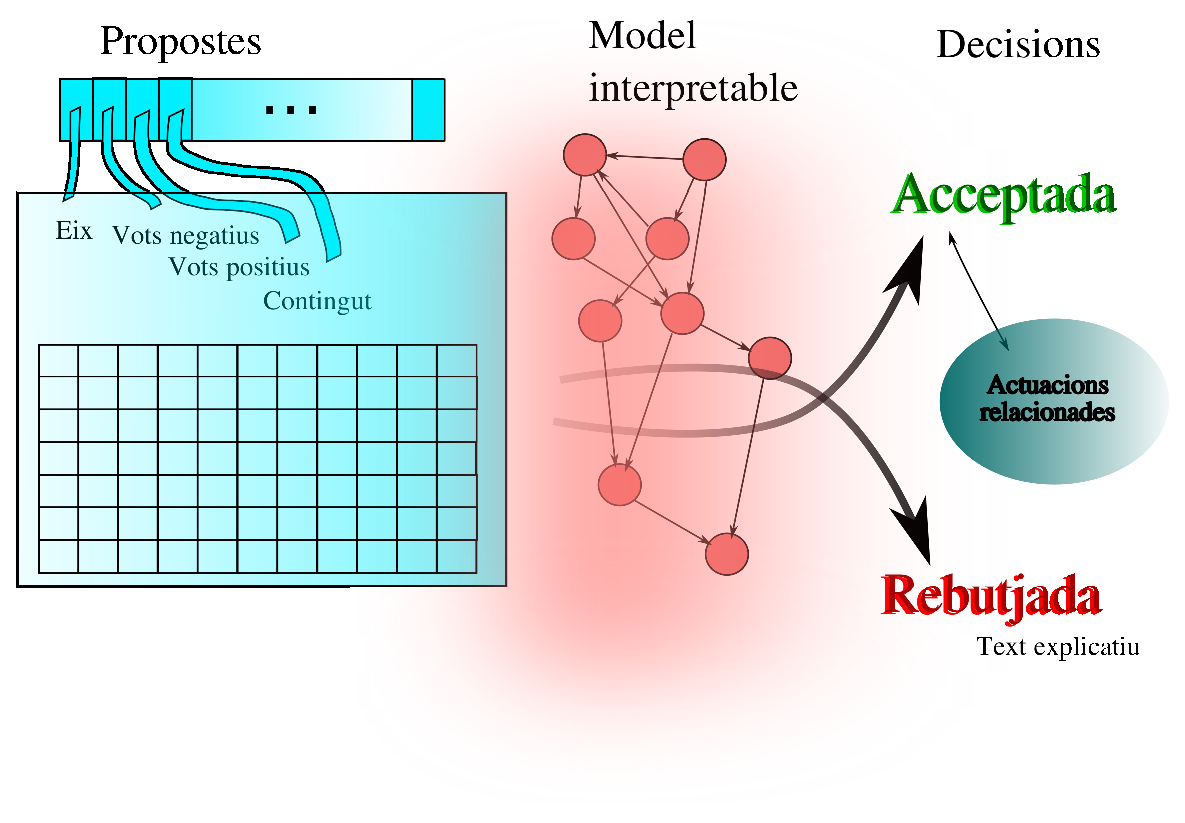
\includegraphics[width=.7\textwidth]{Figures/task.eps}
\caption{Learning the association between proposals and decisions.
The red central part corresponds to the predictive model that we learn from the data observed in the platform \texttt{decidim.barcelona}, which are the list of proposal features for each proposal (in blue, left) and whether the proposal was accepted or not (decision, right).}
\label{fig:task}
\end{figure}

The model that we aim to develop is relevant in the modern society for several reasons. First, generating mathematical models that are able to explain in an objective way which characteristics have more influence on the decision making process of a government team which advocates for transparency, and second, addresses one of the main challenges of giving a good use of the large amounts of data that our society generates.  

\section{Structure of the Report}

First, we will introduce the dataset we will work with and perform a global statistical analysis of all features selected to to gain knowledge about the PAM process. Later on, we will move into applying this knowledge into an interpretable machine learning algorithm, and how we proceeded methodologically. Further on results will be presented and discussed, analyzing the performance of the methods, the information that we are able to retrieve and how insightful conclusions we can draw.Finally, a discussion about the results and what can be improved as well as some further work
ideas.

\newpage


